\chapter{事件表的数据分析}
\label{chap:07}

\begin{chapteropening}
第 \ref{chap:06} 章说明了望远镜怎样把光子候选写成带时间、通道、波长、偏振和质量标记的事件表。现在的问题是：怎样从这张表中得到可检验的科学量？同一份事件表可以投影成光变曲线，可以构造延迟直方图，也可以拟合二阶相关峰、平方可见度或脉冲到达时刻。分析层的选择决定了哪些信息被保留，哪些信息被平均掉。

本章从一个原则出发：先明确数据向量和概率模型，再计算估计量。Iqueye/AquEYE 的光子时间标签、VERITAS-SII 的离线 FPGA 相关、MAGIC-SII 的 GPU 实时 Pearson 相关，以及 Bayesian Blocks 和 Poisson likelihood 的天文统计框架，处理的都是同一个问题：怎样把事件表里的时间和通道信息变成带误差、可复现、可拟合的科学量 \citep{2009A&A...508..531N,2009JMOp...56..261B,2020NatAs...4.1164A,2024MNRAS.529.4387A,1979ApJ...228..939C,2013ApJ...764..167S}。
\end{chapteropening}

\section{事件表先变成概率模型}

沿用第 \ref{chap:06} 章的原始和标定事件表，分析层把一份标定后的事件表简写为
\begin{equation}
  \mathcal{D}
  =
  \left\{
  t_q,\ a_q,\ d_q,\ c_q,\ p_q,\ w_q,\ f_q
  \right\}_{q=1}^{N_{\rm evt}},
  \label{eq:ch07-event-data}
\end{equation}
\begin{formulaexplain}
\(\mathcal D\) 是标定后的事件表；每个 \(q\) 事件保留时间、站点、探测器、光谱、偏振、权重和质量标记；\(N_{\rm evt}\) 是事件总数。它是后续所有估计量的原始数据向量。
\end{formulaexplain}
\(t_q\) 是统一时间尺度上的到达时刻，单位秒；\(a_q\) 是望远镜或站点编号；\(d_q\) 是探测器通道；\(c_q\) 是光谱通道；\(p_q\) 是偏振通道；\(w_q\) 是权重；\(f_q\) 是质量标记。这些字段的仪器来源、时钟校正和格式要求分别见式 \eqref{eq:ch06-raw-event}、\eqref{eq:ch06-calibrated-time} 和第 \ref{chap:06} 章末的数据格式讨论。

分析的第一步不是画图，而是定义选择函数：
\begin{equation}
  S_q =
  S(t_q,a_q,d_q,c_q,p_q,f_q),
  \qquad
  S_q \in \{0,1\}\ {\rm or}\ [0,1].
  \label{eq:ch07-selection}
\end{equation}
\begin{formulaexplain}
\(S_q\) 是第 \(q\) 个事件的选择函数；自变量是事件时间、通道和质量标记。取 0/1 时表示剔除或保留，取连续值时表示曝光、背景或效率权重。
\end{formulaexplain}
二值 \(S_q\) 表示保留或剔除，连续 \(S_q\) 表示曝光、死时间、云量、背景或通道效率带来的权重。若一个通道事件率是 \(10^6\,{\rm s^{-1}}\)，1 小时观测就有 \(3.6\times10^9\) 个事件；此时任何“看图后手动删点”的做法都无法复现。选择函数需要能由元数据和阈值重新生成，后面的光变、相关和拟合都应使用同一套选择。

对未分箱事件，最直接的模型是非齐次 Poisson 点过程。若事件率模型为 \(\lambda(t,\mathbf{x}\mid\boldsymbol{\theta})\)，其中 \(\mathbf{x}\) 代表通道、波长、偏振或天空位置，似然为
\begin{equation}
  \ln L(\boldsymbol{\theta})
  =
  \sum_{q:S_q>0}
  \ln \lambda(t_q,\mathbf{x}_q\mid\boldsymbol{\theta})
  -
  \int_{\mathcal{T}}
  \lambda(t,\mathbf{x}\mid\boldsymbol{\theta})\,E(t,\mathbf{x})\,dt\,d\mathbf{x}.
  \label{eq:ch07-point-process-likelihood}
\end{equation}
\begin{formulaexplain}
\(\ln L\) 是点过程对数似然；\(\lambda\) 是事件率模型，\(\boldsymbol\theta\) 是参数，\(\mathbf x\) 是通道/波长等标签，\(E\) 是有效曝光。第一项奖励事件落在高率处，第二项惩罚预言过多事件。
\end{formulaexplain}
这行式子有两个部分。第一项在每个实际事件处评价模型率：事件落在高率区域会提高似然。第二项是模型在有效曝光 \(E(t,\mathbf{x})\) 上预言的总事件数：模型不能只在事件处很高，还要解释为什么其他时间没有事件。这里 \(\lambda\) 的单位是 s\(^{-1}\) 或 s\(^{-1}\) channel\(^{-1}\)，\(E\) 无量纲或带面积/效率因子，包含坏天气、死时间、通道开关、滤光片透过率和观测窗口。Cash 统计量就是这个 Poisson 似然在 X 射线和低计数天文数据中的经典形式；小计数置信区间不能简单用 \(\sqrt{N}\) 对称误差替代 \citep{1979ApJ...228..939C,1986ApJ...303..336G}。

\begin{figure}[tbp]
\centering
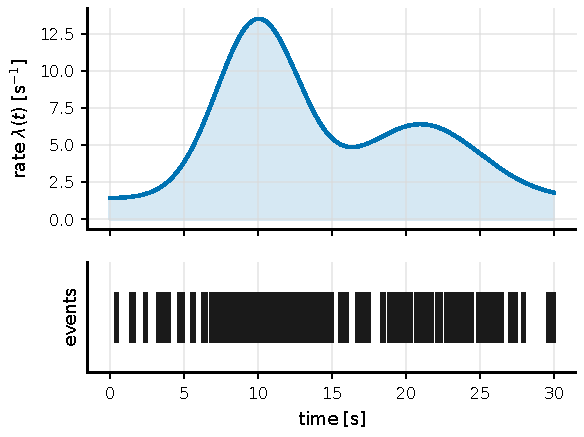
\includegraphics[width=0.72\linewidth]{figures/generated/chapter_07/ch07_poisson_likelihood.pdf}
\caption{非齐次 Poisson 过程的观测图像。上图是瞬时事件率 \(\lambda(t)\)，下图是从该率产生的一组事件时间。似然函数同时使用事件落在高率区域的事实和整段观测的积分率；只把事件重新分箱成一条光变曲线会丢失一部分时间信息，尤其在快速变化和不均匀曝光时更明显。}
\label{fig:ch07-poisson-likelihood}
\end{figure}

如果把事件先分进时间 bin，点过程似然退化为分箱 Poisson 似然：
\begin{equation}
  \ln L
  =
  \sum_i
  \left[
  d_i\ln m_i(\boldsymbol{\theta})
  -m_i(\boldsymbol{\theta})
  -\ln(d_i!)
  \right],
  \label{eq:ch07-binned-poisson}
\end{equation}
\begin{formulaexplain}
\(d_i\) 是第 \(i\) 个 bin 的观测计数，\(m_i\) 是模型计数。这个 Poisson 似然适合分箱后的光变、谱道或延迟直方图，并保留低计数的不对称统计。
\end{formulaexplain}
\(d_i\) 是第 \(i\) 个 bin 的观测计数，\(m_i\) 是模型预言计数，二者都无量纲。这个式子适合光变曲线、延迟直方图和谱道计数；当 \(d_i\gtrsim20\) 且模型远离边界时，常可近似为 Gaussian 似然。若背景、响应矩阵、吸收、时钟漂移或多个模型分量同时存在，似然比检验不一定服从名义上的 \(\chi^2\) 分布；新增分量强度被限制为非负时，零强度位于参数边界，显著性需要用模拟、后验预测检验或明确的模型证据校准 \citep{2002ApJ...571..545P}。

事件表还可以用自适应分段来描述慢变背景或爆发。Bayesian Blocks 把时间轴划成若干常率区间，对事件数据、binned counts 和带误差测量都给出相应的 fitness function；数据空隙通过 live time 进入，而不是被误认为无事件区间 \citep{2013ApJ...764..167S}。在实际管线中，这类方法很适合做质量监控、背景分段和暂现源候选筛选；最终物理参数仍应由明确的模型似然给出。

\Needspace{16\baselineskip}
\section{两路事件怎样给出相关峰}

两路事件表 \(a,b\) 的基本观测量是校正后的时间差：
\begin{equation}
  \tau_{ij}^{ab}
  =
  t_{j,b}^{\rm cal}
  -
  t_{i,a}^{\rm cal}
  -
  \Delta t_{\rm geo}^{ab}(t_i,\hat{\mathbf{s}})
  -
  \Delta t_{\rm inst}^{ab}(t_i).
  \label{eq:ch07-event-delay}
\end{equation}
\begin{formulaexplain}
\(\tau_{ij}^{ab}\) 是站点 \(a,b\) 两个事件的校正延迟；\(t^{\rm cal}\) 是标定时间；\(\Delta t_{\rm geo}\) 和 \(\Delta t_{\rm inst}\) 分别扣除几何和仪器延迟。它决定事件对落入哪个相关 bin。
\end{formulaexplain}
\(t_{i,a}^{\rm cal}\) 和 \(t_{j,b}^{\rm cal}\) 的单位是秒，\(\Delta t_{\rm geo}^{ab}\) 是几何延迟，\(\Delta t_{\rm inst}^{ab}\) 是两通道剩余仪器延迟。对 100 m 基线，几何延迟最大约 333 ns；对 1 km 基线是 \(3.3\,\mu{\rm s}\)。若时间 bin 为 4 ns，几何延迟只要错一个 bin 就会把相关峰移出零延迟；若仪器达到几十皮秒，地球自转导致的投影基线变化也要在短时间块内更新 \citep{2006MNRAS.369..655H,2006MNRAS.372.1549E,2018RNAAS...2....4K,2020NatAs...4.1164A}。

延迟 bin \(k\) 的事件对数为
\begin{equation}
  C_{ab,k}
  =
  \sum_{i\in a}\sum_{j\in b}
  S_iS_j\,
  \mathbf{1}
  \left[
  \tau_k-\frac{\Delta\tau}{2}
  \le
  \tau_{ij}^{ab}
  <
  \tau_k+\frac{\Delta\tau}{2}
  \right],
  \label{eq:ch07-pair-count}
\end{equation}
\begin{formulaexplain}
\(C_{ab,k}\) 是第 \(k\) 个延迟 bin 的事件对数；\(S_iS_j\) 给事件权重；指示函数只选择延迟落在 \(\tau_k\pm\Delta\tau/2\) 内的事件对。它是延迟直方图的基本计数。
\end{formulaexplain}
\(\Delta\tau\) 是延迟 bin 宽，单位秒；\(C_{ab,k}\) 无量纲。若两个通道独立且事件率在活时间内近似稳定，随机符合的期望为
\begin{equation}
  B_{ab,k}
  \simeq
  R_a R_b\,\Delta\tau\,T_{\rm live},
  \label{eq:ch07-accidental}
\end{equation}
\begin{formulaexplain}
\(B_{ab,k}\) 是随机符合背景；\(R_a,R_b\) 是两路平均事件率，\(\Delta\tau\) 是 bin 宽，\(T_{\rm live}\) 是活时间。它给出无天体相关时每个延迟 bin 应有的偶然事件对。
\end{formulaexplain}
\(R_a,R_b\) 的单位是 s\(^{-1}\)，\(T_{\rm live}\) 是扣除坏时间和死时间后的积分时间。典型强度干涉中 \(R_a\) 和 \(R_b\) 可在 \(10^6\)--\(10^8\,{\rm s^{-1}}\)，\(\Delta\tau\) 为 0.1--10 ns，\(T_{\rm live}\) 为分钟到夜级；因此 \(B_{ab,k}\) 可以很大，而天体相关只是这个背景上的 \(10^{-6}\) 到 \(10^{-4}\) 量级超额 \citep{1974iiia.book.....H,2020NatAs...4.1164A,2024MNRAS.529.4387A}。

归一化后的二阶相关估计量写成
\begin{equation}
  \widehat{g}^{(2)}_{ab}(\tau_k)
  =
  \frac{C_{ab,k}}{B_{ab,k}},
  \qquad
  \widehat{C}_{ab}(\tau_k)
  =
  \widehat{g}^{(2)}_{ab}(\tau_k)-1.
  \label{eq:ch07-g2-estimator}
\end{equation}
\begin{formulaexplain}
\(\widehat g^{(2)}\) 是归一化二阶相关估计；\(C_{ab,k}\) 是观测事件对数，\(B_{ab,k}\) 是随机背景；\(\widehat C_{ab}\) 是相对随机背景的超额。强度干涉信号就在这个超额里。
\end{formulaexplain}
\(\widehat{C}_{ab}\) 无量纲。若使用连续波形而不是离散事件，MAGIC-SII 采用 Pearson 相关
\begin{equation}
  \rho_{ab}(\tau_k)
  =
  \frac{\sum_n
  \left[x_a(t_n)-\bar{x}_a\right]
  \left[x_b(t_n+\tau_k)-\bar{x}_b\right]}
  {\sqrt{\sum_n\left[x_a(t_n)-\bar{x}_a\right]^2
  \sum_n\left[x_b(t_n)-\bar{x}_b\right]^2}},
  \label{eq:ch07-pearson}
\end{equation}
\begin{formulaexplain}
\(\rho_{ab}\) 是两路连续波形的 Pearson 相关；\(x_a,x_b\) 是采样电压或电流，\(\bar x\) 是平均值。它衡量去均值后的同步涨落，但还需背景和通量标定才变成 \(|V|^2\)。
\end{formulaexplain}
\(x_a\) 和 \(x_b\) 是数字化电压或电流样本。这个量在硬件里容易实时计算，但它包含恒星、夜天光和电子噪声的混合贡献，还要用直流电流、背景像素和零基线标定转换成 \(|V|^2\) \citep{2024MNRAS.529.4387A}。

\begin{figure}[tbp]
\centering
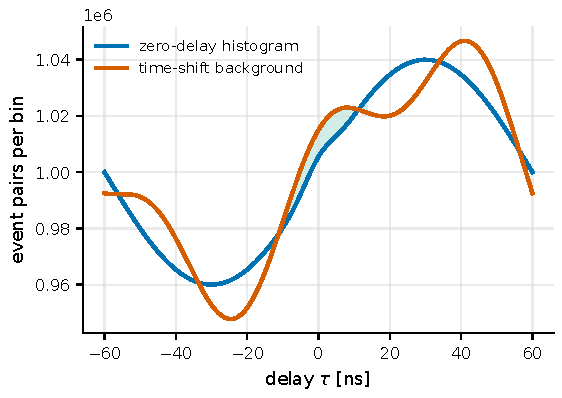
\includegraphics[width=0.72\linewidth]{figures/generated/chapter_07/ch07_time_shift_background.pdf}
\caption{时移背景估计的结构。蓝线是零延迟附近的事件对直方图，橙线是把一个通道整体平移到非物理延迟后得到的 accidental background。绿色区域表示中央相关峰相对时移背景的超额。这个方法可以保留慢变率、坏时间和背景结构，但平移量要远大于仪器响应宽度和天体相关宽度。}
\label{fig:ch07-time-shift-background}
\end{figure}

实际管线通常不用式 \eqref{eq:ch07-accidental} 直接归一化，而是用时间滑移、off-source、off-band 或错偏振估计 \(B_{ab,k}\)。时间滑移把通道 \(b\) 整体平移 \(\Delta T_{\rm shift}\)，要求 \(|\Delta T_{\rm shift}|\) 远大于相关峰宽，却小于背景和增益慢变时间。多个正负滑移可以给出背景均值和背景不确定度。off-source 适合夜天光和暗电流估计，off-band 适合谱线科学，错偏振适合寻找偏振串扰。VERITAS-SII 在 1 s 相关帧上剔除高频电子噪声和低 PMT 电流帧，再对几何延迟校正后的帧加权平均；MAGIC-SII 同时使用信号像素和背景像素的 DC 读数修正夜天光 \citep{2020NatAs...4.1164A,2024MNRAS.529.4387A}。

bin 宽 \(\Delta\tau\) 要和相关峰宽、时间戳量化和最终拟合方式一起选。若 \(\Delta\tau\) 远大于相关峰宽，峰高会被平均稀释；若它远小于时间戳量化和响应函数宽度，相邻 bin 会强相关，计算量也会上升。若最终只拟合峰面积，过细分箱不会增加总信息。对 VERITAS-SII，相关 lag 间隔为 4 ns，峰宽固定在约 4 ns；对 80 ps TDC 和几十皮秒探测器，bin 可以更细，但几何延迟、仪器响应和时钟残差也要同等精度 \citep{2020NatAs...4.1164A,2020RScI...91a3108W,2009A&A...508..531N}。

\section{相关器怎样在可承受时间内工作}

直接双循环计算式 \eqref{eq:ch07-pair-count} 的复杂度是 \(O(N_aN_b)\)。若两路各有 \(10^9\) 个事件，全量比较需要 \(10^{18}\) 次差分，不可能作为常规分析。排序窗口算法先按时间排序，只在 \(|t_{j,b}-t_{i,a}|\le W\) 的窗口内找事件对：
\begin{equation}
  N_{\rm pair}^{\rm win}
  \simeq
  2W\,R_b\,N_a .
  \label{eq:ch07-window-pairs}
\end{equation}
\begin{formulaexplain}
\(N_{\rm pair}^{\rm win}\) 是窗口算法需要检查的候选事件对数；\(W\) 是延迟窗口半宽，\(R_b\) 是第二路事件率，\(N_a\) 是第一路事件数。有限窗口把复杂度从全量双循环大幅降下来。
\end{formulaexplain}
\(W\) 是最大延迟窗口半宽，单位秒。如果 \(W=100\,{\rm ns}\)、\(R_b=10^6\,{\rm s^{-1}}\)、\(N_a=10^9\)，候选对约 \(2\times10^8\)，比全量双循环少十个数量级。这个算法适合稀疏事件表，也适合保留每个事件的波长和偏振标签。

若已经把事件或电压流放进均匀时间 bin，可用 FFT 计算互相关：
\begin{equation}
  c_{ab}[k]
  =
  \mathcal{F}^{-1}
  \left[
  \mathcal{F}\{x_a[n]\}^{*}
  \mathcal{F}\{x_b[n]\}
  \right]_k .
  \label{eq:ch07-fft-correlation}
\end{equation}
\begin{formulaexplain}
\(c_{ab}[k]\) 是离散互相关；\(\mathcal F\) 和 \(\mathcal F^{-1}\) 是 Fourier 变换与反变换；星号表示复共轭。FFT 把时域互相关改写成频域乘法，适合均匀采样数据。
\end{formulaexplain}
\(x_a[n]\) 和 \(x_b[n]\) 是时间序列，\(\mathcal{F}\) 是离散 Fourier 变换。FFT 方法的复杂度约 \(O(M\log M)\)，\(M\) 是时间 bin 数；它适合连续采样和固定 bin 的高速相关，但一旦分箱完成，低于 bin 宽的时间信息就不能恢复。VERITAS-SII 把连续 PMT 信号流到磁盘后用 FPGA 离线相关；MAGIC-SII 用 GPU 在观测时实时计算四通道所有成对相关；多通道 TCSPC 输出按时间排序的事件流，便于离线构造任意延迟和通道选择 \citep{2020NatAs...4.1164A,2024MNRAS.529.4387A,2020RScI...91a3108W}。

\begin{figure}[tbp]
\centering
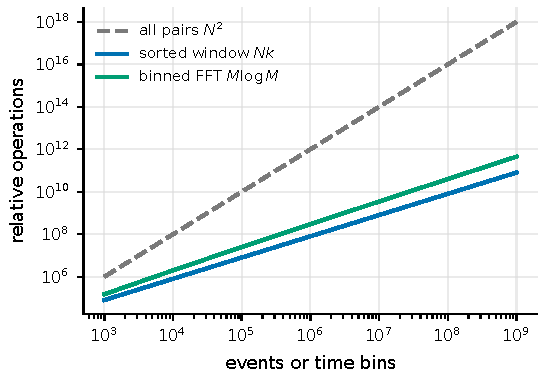
\includegraphics[width=0.72\linewidth]{figures/generated/chapter_07/ch07_correlator_scaling.pdf}
\caption{三类相关计算的操作数标度。全量事件对双循环随 \(N^2\) 增长，只适合小样本或教学检验；排序窗口算法只比较有限延迟内的事件对，接近线性增长；均匀分箱后的 FFT 相关随 \(M\log M\) 增长，适合连续采样或实时质量监控。实际速度还取决于内存带宽、I/O、GPU/FPGA 数据布局和质量标记筛选。}
\label{fig:ch07-correlator-scaling}
\end{figure}

算法选择会反过来影响科学量。排序窗口保留每个事件的全部标签，适合后验重新筛选；FFT 相关速度快，适合固定通道和固定时间 bin；实时 FPGA/GPU 相关可以在观测中发现时钟跳变、电子串扰和云导致的通量突变，但通常只保存压缩后的相关产品。对长期归档，原始事件或原始波形、标定事件、相关产品最好同时保存；FITS BINTABLE 适合事件归档，HDF5/Parquet 适合列式大数据分析，Astropy 可处理 FITS、时间和坐标元数据 \citep{2010A&A...524A..42P,2013A&A...558A..33A,2018AJ....156..123A}。

\section{误差为什么不是一串独立误差棒}

若 \(C_{ab,k}\) 和 \(B_{ab,k}\) 都是独立 Poisson 计数，且背景由 \(M\) 个等权时间滑移估计，则中央超额的近似方差为
\begin{equation}
  \operatorname{Var}
  \left[
  C_{ab,k}-\widehat{B}_{ab,k}
  \right]
  \simeq
  C_{ab,k}
  +
  \frac{1}{M}B_{ab,k}.
  \label{eq:ch07-excess-variance}
\end{equation}
\begin{formulaexplain}
\(\operatorname{Var}\) 是中央超额的方差；\(C_{ab,k}\) 给信号窗口的 Poisson 噪声，\(B_{ab,k}/M\) 给 \(M\) 个滑移背景平均后的不确定度。它是独立计数近似下的误差预算。
\end{formulaexplain}
这个近似只在事件独立、滑移背景互不重叠且率稳定时成立。真实数据里，相邻延迟 bin 共享事件，多个基线共享同一望远镜，多个波长通道共享天气和增益，多个模型点共享零基线归一化，因此误差通常不是对角的。

完整数据向量可以写为
\begin{equation}
  \mathbf{d}
  =
  \left(
  \widehat{|V|^2}_{1},
  \widehat{|V|^2}_{2},
  \ldots,
  \widehat{|V|^2}_{N_d}
  \right),
  \qquad
  \Sigma_{ij}
  =
  \left\langle
  (d_i-\mu_i)(d_j-\mu_j)
  \right\rangle .
  \label{eq:ch07-covariance}
\end{equation}
\begin{formulaexplain}
\(\mathbf d\) 是相关产品数据向量；\(d_i\) 是第 \(i\) 个 \(|V|^2\) 数据点，\(\mu_i\) 是其均值；\(\Sigma_{ij}\) 是协方差。非对角项记录共享望远镜、背景或标定带来的相关误差。
\end{formulaexplain}
\(\Sigma_{ij}\) 的单位是数据量单位的乘积；若 \(d_i\) 是无量纲 \(|V|^2\)，\(\Sigma\) 也无量纲。协方差可由解析误差传播、时间块 bootstrap、jackknife、时移背景集合或端到端注入仿真估计。时间块长度要长于相关峰宽、电子噪声相关时间和指向/天气短时波动；对夜级数据，常用 10 s 到数分钟的块来测试误差是否随 \(T^{-1/2}\) 收敛。MAGIC-SII 把电子带宽、光学带宽、DC 读出增益、背景扣除和残余电子噪声列为系统项，并通过改变 \(|V|^2\) 数据点的极端方向估计角直径系统误差 \citep{2024MNRAS.529.4387A}。

\begin{figure}[tbp]
\centering
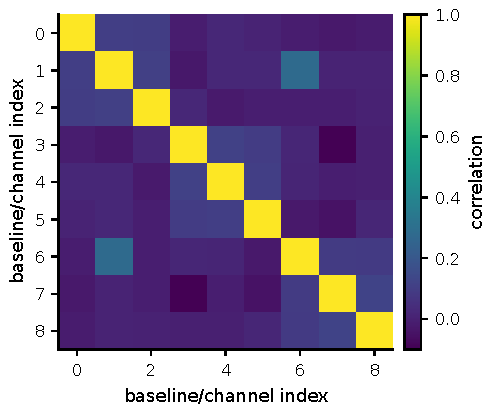
\includegraphics[width=0.66\linewidth]{figures/generated/chapter_07/ch07_covariance_matrix.pdf}
\caption{多基线或多通道结果的协方差矩阵示意。对角项是单个数据点方差，邻近块来自同一时间段或同一望远镜共享的噪声，远离对角线的结构可能来自共同背景估计、零基线归一化或电子串扰。模型拟合若只使用对角误差，会把有效独立信息量估得过高。}
\label{fig:ch07-covariance-matrix}
\end{figure}

空检验要和主分析使用同一套选择函数和权重。常用检验包括：把一个通道平移到非物理延迟；交换正负几何延迟；使用两个不应相关的偏振或波长通道；把目标外天空作为背景；把望远镜对分成不同时间块；把单个望远镜或单夜数据逐一剔除；在真实事件表中注入已知相关峰并检查能否无偏恢复。若主信号只在某个选择阈值下出现，而在相邻阈值、错延迟或 jackknife 中消失，它更可能是管线选择或仪器状态的结果，而不是天体相关。

\section{怎样从相关产品得到物理参数}

相关函数估计完成后，常见模型是把角直径、双星分离、亮度比、环半径或喷流参数映射到平方可见度：
\begin{equation}
  \mathbf{m}(\boldsymbol{\theta})
  =
  \left[
  |V(\mathbf{u}_1,\lambda_1\mid\boldsymbol{\theta})|^2,
  \ldots,
  |V(\mathbf{u}_{N_d},\lambda_{N_d}\mid\boldsymbol{\theta})|^2
  \right].
  \label{eq:ch07-model-vector}
\end{equation}
\begin{formulaexplain}
\(\mathbf m(\boldsymbol\theta)\) 是物理模型预言的数据向量；每一项是在对应空间频率 \(\mathbf u_i\) 和波长 \(\lambda_i\) 处的 \(|V|^2\)。它把角直径、双星参数或结构参数映射到观测量。
\end{formulaexplain}
\(\mathbf{u}=\mathbf{B}_\perp/\lambda\) 是空间频率，单位 rad\(^{-1}\) 或以波长为单位的投影基线；\(\boldsymbol{\theta}\) 是物理参数。若 \(\mathbf{d}\) 已经是近似 Gaussian 的相关产品，似然可写为
\begin{equation}
  -2\ln L
  =
  \left[\mathbf{d}-\mathbf{m}(\boldsymbol{\theta})\right]^T
  \Sigma^{-1}
  \left[\mathbf{d}-\mathbf{m}(\boldsymbol{\theta})\right]
  +\ln |\Sigma| + {\rm const}.
  \label{eq:ch07-gaussian-likelihood}
\end{equation}
\begin{formulaexplain}
\(\mathbf d-\mathbf m\) 是数据和模型残差；\(\Sigma^{-1}\) 按协方差加权；\(\ln|\Sigma|\) 是协方差归一化项。它是带相关误差的数据产品常用 Gaussian 似然。
\end{formulaexplain}
如果直接拟合原始计数或低计数延迟 bin，应回到式 \eqref{eq:ch07-binned-poisson}。VERITAS-SII 用均匀圆盘和边缘昏暗模型拟合 \(|g^{(1)}|^2\) 随投影基线的变化；MAGIC-SII 把 Pearson 相关经通量和背景校准后得到 \(|V|^2\)，再拟合恒星角直径和系统误差 \citep{2020NatAs...4.1164A,2024MNRAS.529.4387A,1967MNRAS.137..375H}。

观测设计阶段常用 Fisher 矩阵估计参数误差：
\begin{equation}
  F_{\alpha\beta}
  =
  \frac{\partial \mathbf{m}^T}{\partial \theta_\alpha}
  \Sigma^{-1}
  \frac{\partial \mathbf{m}}{\partial \theta_\beta},
  \qquad
  \operatorname{Cov}(\theta_\alpha,\theta_\beta)
  \gtrsim
  (F^{-1})_{\alpha\beta}.
  \label{eq:ch07-fisher}
\end{equation}
\begin{formulaexplain}
\(F_{\alpha\beta}\) 是 Fisher 信息矩阵；导数描述模型对参数的敏感度，\(\Sigma^{-1}\) 给误差权重；\(F^{-1}\) 近似给参数协方差下界。它用于观测规划和高信噪比误差估计。
\end{formulaexplain}
\(F_{\alpha\beta}\) 的单位是 \(\theta_\alpha^{-1}\theta_\beta^{-1}\)。若误差只由独立光子统计决定，信息量通常随有效光子数近似线性增加，参数误差随 \(N_{\rm eff}^{-1/2}\) 降低；一旦电子带宽、背景扣除、零基线归一化或通道增益给出系统地板，继续积分只会让误差趋近地板。Fisher 矩阵来自局部二次近似，适合观测规划和高信噪比近似；多峰后验、非线性退化或参数边界需要 MCMC、nested sampling 或端到端模拟 \citep{1925PCPS...22..700F,2013PASP..125..306F,2009MNRAS.398.1601F}。

\begin{figure}[tbp]
\centering
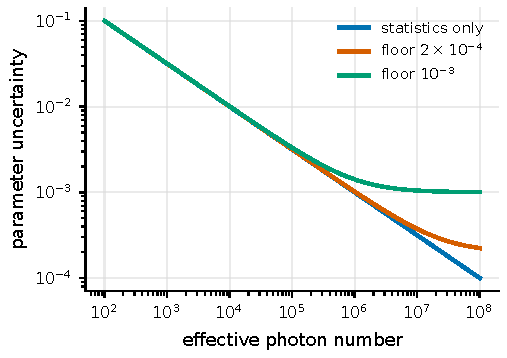
\includegraphics[width=0.70\linewidth]{figures/generated/chapter_07/ch07_fisher_scaling.pdf}
\caption{参数误差随有效光子数增加的标度。蓝线是纯统计 \(N_{\rm eff}^{-1/2}\) 下降；橙线和绿线加入不同系统误差地板后，长时间积分不再改善最终误差。观测计划应把积分时间、目标亮度、基线覆盖和系统标定放在同一个误差预算里。}
\label{fig:ch07-fisher-scaling}
\end{figure}

贝叶斯后验写成
\begin{equation}
  p(\boldsymbol{\theta}\mid\mathcal{D},M)
  =
  \frac{
  L(\mathcal{D}\mid\boldsymbol{\theta},M)\,
  \pi(\boldsymbol{\theta}\mid M)}
  {Z_M},
  \qquad
  Z_M=
  \int
  L\,\pi\,d\boldsymbol{\theta}.
  \label{eq:ch07-posterior}
\end{equation}
\begin{formulaexplain}
\(p(\boldsymbol\theta\mid\mathcal D,M)\) 是模型 \(M\) 下的参数后验；\(L\) 是似然，\(\pi\) 是先验，\(Z_M\) 是证据。它把数据约束和外部物理先验合成完整的不确定度描述。
\end{formulaexplain}
\(\pi\) 是先验，\(Z_M\) 是模型证据。先验可以来自距离、光谱型、已有角直径、双星轨道、爆发时间或物理边界；它需要写清楚，因为强度干涉常只测 \(|V|^2\)，缺少相位会让镜像、亮度比和位置角出现退化。emcee 适合中等维度后验采样，MultiNest 适合多峰后验和模型证据估计；二者都不能替代物理检查，链的自相关时间、接受率、先验体积和模拟注入恢复都要报告 \citep{2013PASP..125..306F,2009MNRAS.398.1601F,1992ApJ...398..146G}。

